\section{APPENDIX}

\subsection{Finger model data}
$F_0 = (123.0, 219.0, 23.52, 91.74,	21.6, 124.8, 129.6)$\\
$
JR = 
\begin{pmatrix}
-0.08941 & -0.0447 & -0.009249 & 0.03669 & 0.1421 & 0.2087 & -0.2138 \\
-0.04689 & -0.1496 & 0.052 &0.052 & 0.0248 & 0.0 & 0.0248 \\ 
0.06472 & 0.001953 & -0.1518 &-0.1518 & 0.2919 & 0.0568 & 0.2067 \\
0.003081 & -0.002352 & -0.0001649 & -0.0001649 & -0.0004483 & 0.0001578 & -0.000685
\end{pmatrix}$

$task_x = (1.0,0.0,0.0,0.0)$

$task_y = (0.0,1.0,0.0,0.0)$

Palmar force is $task_z = (0.0,0.0,1.0,0.0)$

%$task_xy = (1.0,1.0,0.0,0.0)$

\begin{figure}[h]
\centering
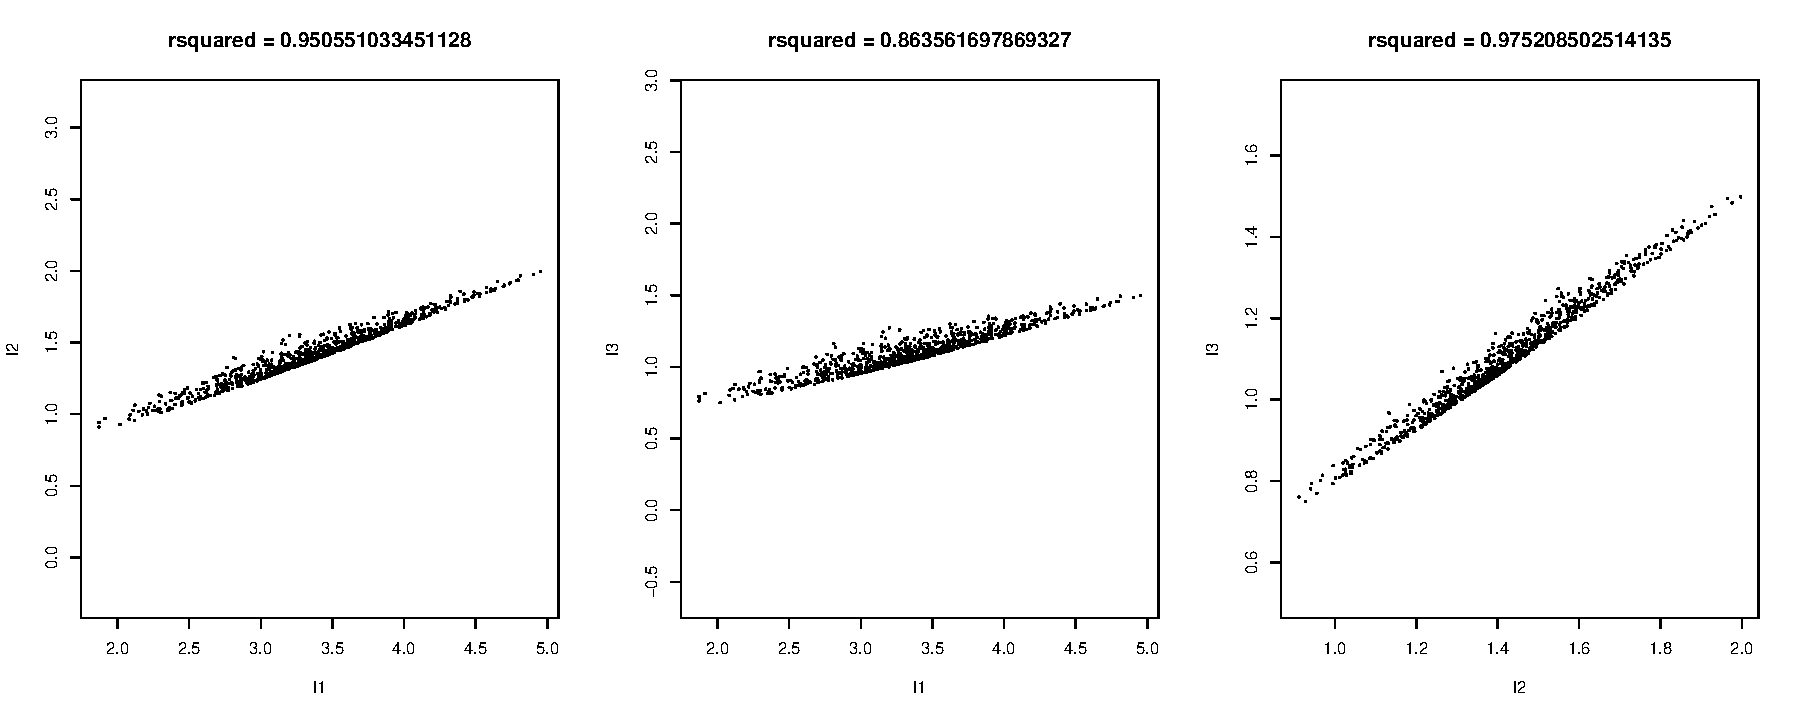
\includegraphics[width=\textwidth,page=1]{figs/cost_function_scatterplots.pdf}
\caption{Non weighted cost functions}
\label{fig:unweighted_cost_functions}
\end{figure}

\begin{figure}[h]
\centering
\includegraphics[width=\textwidth,page=2]{figs/cost_function_scatterplots.pdf}
\caption{Weighted cost functions}
\label{fig:weighted_cost_functions}
\end{figure}
% R code to compute the pdf: \\ fixed_db <- the data\\ ecdf(fixed_db[fixed_db['alpha']==0.9,][,3])(c(0.49,0.51))\\